\section{Current Sensing}
To address the difficulties of creating an accurate current-measurement circuit for cost-effective applications, designers have a variety of choices at their disposal. The best flexibility is provided by using general-purpose operational amplifiers (op amps) or analog-to-digital converters (ADCs), they could be standalone or embedded in a microcontroller (MCU). While also leveraging a wide range of tailored components that are specifically made for current sensing but also address challenges in a specific way \cite{TI_Current_Sensing}.
Shunt resistors(Kelvin method) and/or hall sensors are the two methods more widely used methods in automotive BMS applications to measure the battery pack current(Charging/Discharging and Balancing current). The integrated solutions for measuring current is more preferable, to secure the space and power constraints in automotive applications. The following sections will give more insights into the current sense methods.

\section{Hall Effect Current Sensors }
"The Hall effect is the creation of a voltage difference (the Hall voltage) across an electrical conductor that is transverse to an applied magnetic field perpendicular to the current and an electric current in the conductor". Well, that is a bit of a more scientific and deep mathematical explanation of the Hall effect. If I take a little leverage to explain the Hall effect in the nomenclature The Current flow in the conductor causes to induce magnetic flux inside the magnetic core, these fluxes also turn out a small potential, which can be called hall voltage. The Hall voltage dropped across the coil (Magnetic) is directionally proportional to the current flowing in the conductor.
A galvanically isolated Hall effect current sensor capable of DC or AC measurement with high accuracy, excellent linearity, and temperature stability\cite{TI_Hall_Current_Sensing_TMCS1107}.
Let us explore hall sensors with some typical examples in the BMS such as the TMCS1107xx \cite{TI_Hall_Current_Sensing_TMCS1107} series from the TI are the most popular and competitive galvanic solutions for measuring the current.

\subsection{TMCS1107xx Sensors :}
The TMCS1107-Q1 is a galvanically isolated Hall effect current sensor with high accuracy, great linearity, and temperature stability for measuring DC or AC currents. A signal chain with low drift and temperature compensation offers a $3\%$ full-scale error over the device temperature range.\\
A magnetic field is created by the input current flowing through an internal 1.8-m conductor, which is monitored by an integrated Hall-effect sensor. This topology reduces design complexity and does away with external concentrators. Reduced conductor resistance decreases thermal and power loss. A 420-V lifetime working voltage and a 3-kV RMS minimal isolation between the current path and circuitry are provided by inherent galvanic insulation. Transient immunity and high common-mode rejection are made possible by integrated electrical shielding. \\
The output voltage is proportional to the input current. Fixed sensitivity minimizes ratiometry errors and enhances supply noise rejection, enabling the TMCS1107-Q1 to run from a single 3-V to 5.5-V power supply. When current enters the positive input pin, it is regarded as having a positive polarity. There are options for both unidirectional and bidirectional sensing.\\
\begin{figure}[h]
	\centering
	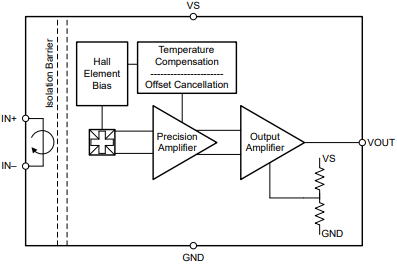
\includegraphics[width=0.6\textwidth]{Chap05/Figures/TMCS1107_HallSensor.PNG}
	\caption{TMCS1107xx Hall sensor Block diagram} 
	\label{fig:TMCS1107xx Hall sensor Block diagram}
\end{figure}
Input current to the TMCS1107-Q1 passes through the isolated side of the package lead frame through the
IN+ and IN– pins. The current flow through the package generates a magnetic field that is proportional to the
input current and measured by a galvanically isolated, precision, Hall sensor IC. As a result of the electrostatic
shielding on the Hall, sensor die, only the magnetic field generated by the input current is measured, thus limiting
input voltage switching pass-through to the circuitry\cite{TI_Hall_Current_Sensing_TMCS1107}.

\section{Shunt Resistors for Battery Current Measurement}
Sensing the voltage drop across a shunt or current-sense resistor \ref{fig:INA_high_side_currentsense} to determine the current in the most typical way. It is necessary to look at the parametric values of both the resistor and current-sense amplifier to obtain a very precise measurement of the current.
Accuracy loss must be prevented by carefully planning the connections between the current-sense amplifier and the resistor.
\begin{figure}[h]
	\centering
	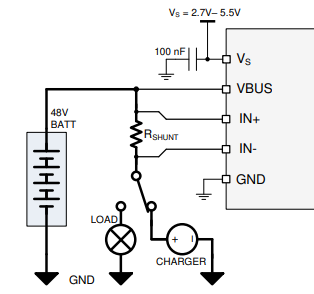
\includegraphics[width=0.4\textwidth]{Chap05/Figures/INA_high_side_currentsense.PNG}
	\caption{ INA238 High-Side Shunt Current Sensing} 
	\label{fig:INA_high_side_currentsense}
\end{figure}

INA2XX series shunt current sensors are the most competitive solution offered by TI to measure the high-side and low-side shunt current with high precision. INA238 is used in this project to measure the shunt current, bus voltage, and several other parameters. Section \ref{sec:INA238} will talk extensively about the INA238 and the features offered by the sensor to synchronize current measurements for BMS application.
\section{INA238/INA2xx}\label{sec:INA238}
The INA238 is a 16-bit delta-sigma ADC with an ultra-precise digital power monitor that is made primarily for current-sensing applications. With a common-mode voltage support range of -0.3 V to +85 V, the device can measure a full-scale differential input of $\pm$163.84 mV or $\pm$40.96 mV via a resistive shunt sensing element.
The INA238 does the necessary calculations in the background while reporting current, bus voltage, temperature, and power. The embedded temperature sensor is useful for tracking the system's ambient temperature and has a die temperature measurement accuracy of 1°C.

The INA238 can be utilized in accurate systems without undergoing multi-temperature calibration during production thanks to its low offset and gain drift design. Additionally, a wide dynamic range is provided without considerable power dissipation losses on the sensing shunt element thanks to the extremely low offset voltage and noise. This enables use in A to kA sensing applications. Due to the device's low input bias current, bigger current-sense resistors can be used, resulting in precise current readings in the micro-amp range.
The device supports samples averaging from 1x to 1024x and adjustable ADC conversion durations from 50$\mu$ s to 4.12 ms, which further reduces noise in the measured data.

\begin{figure}[h]
	\centering
	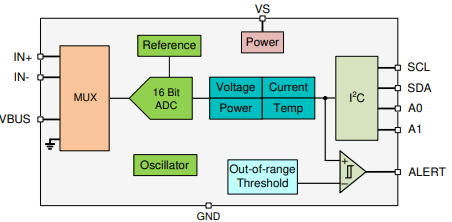
\includegraphics[width=0.6\textwidth]{Chap05/Figures/INA238_Simplified_Block_diagram.PNG}
	\label{fig:INA238_Simplified_Block_diagram}
	\caption{INA238 Simplified Block diagram \cite{INA238_User_Datasheet}}
\end{figure}

The INA238 has a multifunctional, open-drain ALERT output pin that can be utilized to report various problems or as a sign that the ADC conversion is finished while the device is functioning in both triggered and continuous conversion mode. Every time an output value under continuous monitoring exceeds its corresponding out-of-range threshold, the diagnostics mentioned in Table 7 can be transmitted via the ALERT pin.

% \begin{table}[h]
%     \centering
%     \begin{tabular}{|l|l|l|}
%     \hline
% 		INA238 DIAGNOSTIC & STATUS BIT ALRT REGISTER (RO) & OUT-OF-RANGE THRESHOLD REGISTER (R/W)  \\ \hline
%         Shunt Under Voltage Limit & SHNTUL & SUVL\\ \hline
%         Shunt Over Voltage Limit & SHNTOL & SOVL \\ \hline
%         Bus Voltage Over-Limit & BUSOL & BOVL \\ \hline
%         Bus Voltage Under-Limit & BUSUL & BUVL \\ \hline
%         Temperature Over-Limit & TMPOL & TEMP\_LIMIT \\ \hline
%         Power Over-Limit & POL & PWR\_LIMIT & 0x7FFF H \\ \hline
%     \end{tabular}
% \end{table}

The diagnosis that prompted the ALERT pin can be identified by reading the DIAG ALRT register. In addition to configuring some ALERT pin functions, this register, which is depicted in Table 7, is also utilized to monitor other related diagnostics.

\begin{itemize}
	\item Alert latch enables — In the event that the ALERT pin is activated, this feature will maintain the pin's value even after all diagnostic circumstances have been resolved. The status of the ALERT pin is reset by reading the DIAG ALRT register. By setting the ALATCH bit, this function is made available.
	\item Conversion ready enable —  When an ADC conversion is finished and the output values are prepared to be received through the digital interface, the CONVERTION READY ENABLE signal instructs the ALERT pin to assert. Setting the CNVR bit enables this feature. Regardless of the CNVR bit set, the conversion completed events can also be read through the CNVRF bit.
	\item Alert comparison on averaged output — Enables comparison of the out-of-range threshold value to the ADC's averaged data values. Comparing the output data to the out-of-range threshold, this aids in further removing noise from the data to prevent false alarms brought on by noise. However, because of the time required for averaging, the diagnosis will be postponed. Setting the SLOWALERT bit activates this feature.
	\item Alert polarity — Allows the device to flip the ALERT pin's active state. Keep in mind that the ALERT pin is an open-drain output that requires a resistor to be pulled up. The APOL control bit can be used to change the ALERT pin's default active-low function to an active-high one.
\end{itemize}

Other diagnostic features that the ALERT pin does not report but which can be accessed by checking the DIAG ALRT register include:

\begin{itemize}
	\item Math overflow — The MATHOF bit indicates when an arithmetic operation has resulted in an internal register overflow, which is reported.
	\item Memory status — The MEMSTAT bit, which monitors the non-volatile trim memory of the device, indicates the memory status. When the gadget is functioning properly, this bit should always be set to '1'.
\end{itemize}

The ALERT pin becomes a multifunctional reporting output when set up to report the ADC conversion complete event. In the example shown in Figure \ref{fig:INA238_multi_alert}, the INA238 device reports ADC conversion complete events while also experiencing shunt over-voltage (over current), bus under voltage, over temperature, and overpower limit events.

\begin{figure}
	\centering
	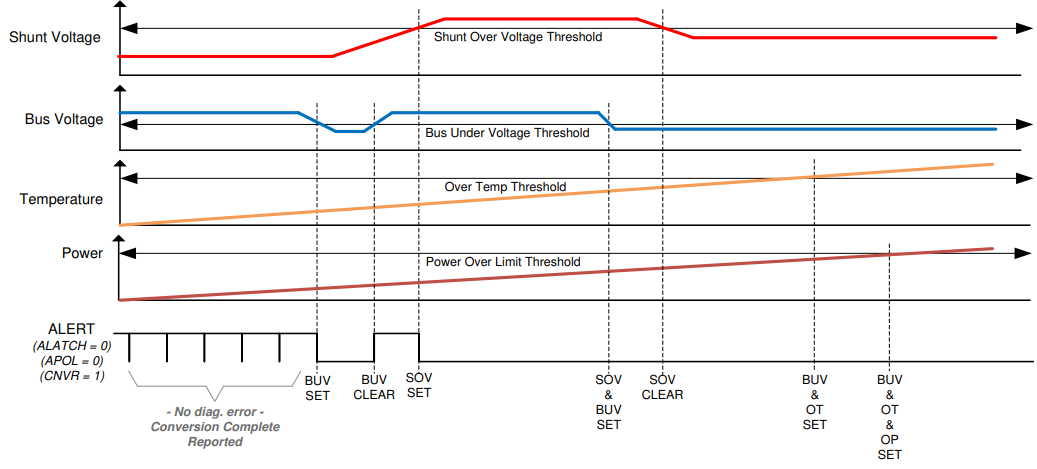
\includegraphics[width=0.8\textwidth]{Chap05/Figures/INA238_multi_alert.PNG}
	\caption{INA238 Multi-Alert Configuration}
	\label{fig:INA238_multi_alert}
\end{figure}